\clearpage\section{V2d robustness battery (v3)}
Spec \path{analysis/v3_spec.md} frozen 2026-10-03T09:52:27Z, first run 09:53:32Z; every check run once; $N_{\text{trials}}$ raised to 132. Results: \path{analysis/output/v3_results.md}. \hfill \tagp

\emph{Reading against the pre-declared rule: fragile in one dimension (R4).} V2d lost money in the first half of the test (Sharpe $-0.21$) and made it in the second ($+0.64$); the other six conditions hold. The 12-month IC is positive in both halves.

\subsection*{R1 Components \hfill \tagp}
{\footnotesize\setlength{\tabcolsep}{4pt}% POST-HOC | source: analysis/output/study2/tables/v3_r1_components.csv (generated by analysis/run.ipynb)
\begin{tabular}{lrrrrr}
\toprule
Sharpe research & Sharpe test & Sharpe full & Test IC 12m (t) & Test alpha t \\
\midrule
+0.41 & +0.19 & +0.27 & +0.093 (+2.90) & +0.79 \\
+0.18 & +0.16 & +0.15 & +0.085 (+1.75) & +0.81 \\
+0.10 & +0.42 & +0.29 & +0.082 (+1.38) & +1.48 \\
+0.11 & +0.16 & +0.13 & +0.032 (+0.87) & +0.69 \\
+0.50 & +0.29 & +0.35 & +0.096 (+2.43) & +1.37 \\
\bottomrule
\end{tabular}
}\par\medskip
\subsection*{R2 Horizon profile \hfill \tagp}
\begin{figure}[H]\centering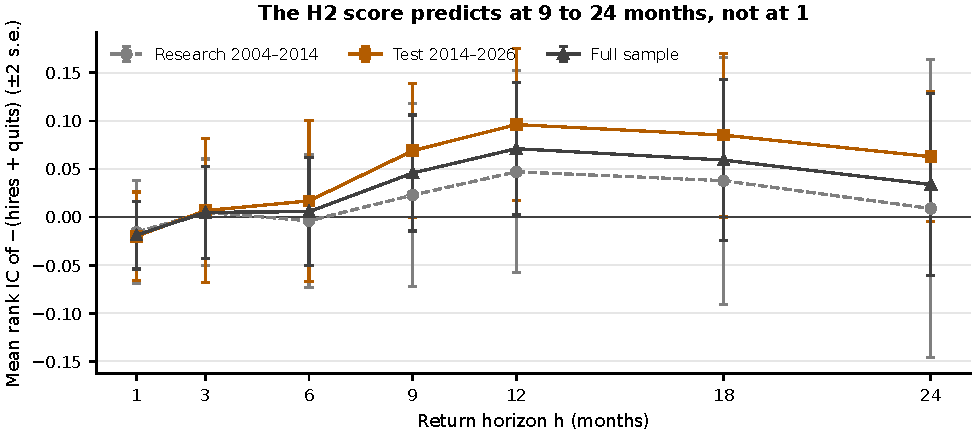
\includegraphics[width=\linewidth]{../report/figures/fig_horizon_profile.pdf}
\caption{The V2d score has no one-month IC and a positive IC from 9 to 24 months, peaking at 12 (test $+0.096$, $t=2.43$). \textcolor{mute}{\footnotesize Source: analysis/output/tables/v3\_r2\_horizon\_profile.csv.} \hfill \tagp}\end{figure}
{\footnotesize\setlength{\tabcolsep}{4pt}% POST-HOC | source: analysis/output/study2/tables/v3_r2_horizon_profile.csv (generated by analysis/run.ipynb)
\begin{tabular}{lrrr}
\toprule
research & test & full \\
\midrule
$-$0.016 ($-$0.59) & $-$0.020 ($-$0.87) & $-$0.019 ($-$1.08) \\
+0.005 (+0.18) & +0.007 (+0.18) & +0.005 (+0.21) \\
$-$0.004 ($-$0.11) & +0.017 (+0.40) & +0.006 (+0.20) \\
+0.023 (+0.48) & +0.069 (+1.98) & +0.046 (+1.52) \\
+0.047 (+0.90) & +0.096 (+2.43) & +0.071 (+2.06) \\
+0.038 (+0.59) & +0.085 (+2.00) & +0.059 (+1.41) \\
+0.009 (+0.11) & +0.063 (+1.86) & +0.034 (+0.72) \\
\bottomrule
\end{tabular}
}\par\medskip
\subsection*{R3 Holding period \hfill \tagp}
\begin{figure}[H]\centering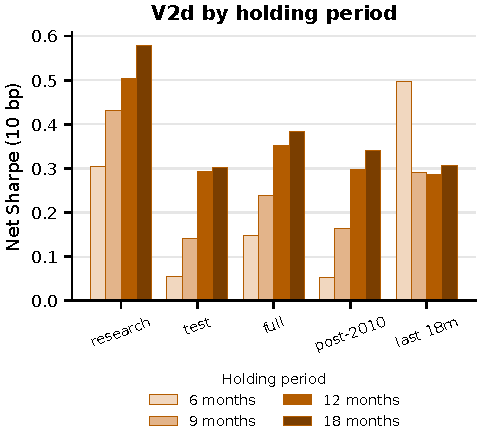
\includegraphics[width=0.55\linewidth]{../report/figures/fig_v2d_holding.pdf}
\caption{Longer holding helps: test Sharpe $+0.05$ at 6 months, $+0.29$ at 12, $+0.30$ at 18. \textcolor{mute}{\footnotesize Source: v3\_r3\_holding.csv.} \hfill \tagp}\end{figure}
{\footnotesize\setlength{\tabcolsep}{4pt}% POST-HOC | source: analysis/output/study2/tables/v3_r3_holding.csv (generated by analysis/run.ipynb)
\begin{tabular}{lrrrrrr}
\toprule
Holding & research & test & full & post-2010 & last 18m & Test turnover \\
\midrule
6 months & +0.31 & +0.05 & +0.15 & +0.05 & +0.50 & 0.49 \\
9 months & +0.43 & +0.14 & +0.24 & +0.16 & +0.29 & 0.40 \\
12 months & +0.50 & +0.29 & +0.35 & +0.30 & +0.29 & 0.37 \\
18 months & +0.58 & +0.30 & +0.38 & +0.34 & +0.31 & 0.28 \\
\bottomrule
\end{tabular}
}\par\medskip
\subsection*{R4 Sub-periods \hfill \tagp}
{\footnotesize\setlength{\tabcolsep}{4pt}% POST-HOC | source: analysis/output/tables/v3_r4_subperiods.csv (generated by analysis/run.ipynb)
\begin{tabular}{lrrrr}
\toprule
Window & Months & Sharpe & Net p.a. & IC 12m (t) \\
\midrule
test: first half & 71 & $-$0.21 & $-$1.4\% & +0.097 (+1.75) \\
test: second half & 71 & +0.64 & +6.5\% & +0.095 (+1.60) \\
test: excl. Mar 2020-Dec 2021 & 120 & +0.37 & +3.0\% & +0.105 (+2.23) \\
test: pre-2020 & 62 & +0.14 & +0.8\% & +0.114 (+1.92) \\
test: 2020 onward & 80 & +0.37 & +3.9\% & +0.080 (+1.54) \\
full: first half & 134 & +0.33 & +2.0\% & +0.038 (+0.73) \\
full: second half & 134 & +0.38 & +3.3\% & +0.107 (+2.66) \\
full: excl. Mar 2020-Dec 2021 & 246 & +0.40 & +2.9\% & +0.073 (+1.93) \\
full: pre-2020 & 188 & +0.36 & +2.2\% & +0.068 (+1.57) \\
\bottomrule
\end{tabular}
}\par\medskip
\subsection*{R5 Costs \hfill \tagp}
{\footnotesize\setlength{\tabcolsep}{4pt}% POST-HOC | source: analysis/output/study2/tables/v3_r5_costs.csv (generated by analysis/run.ipynb)
\begin{tabular}{lrrrrr}
\toprule
Window & 0 bp & 10 bp & 25 bp & 50 bp & Break-even (bp) \\
\midrule
research & +0.58 & +0.50 & +0.39 & +0.20 & 76 \\
test & +0.34 & +0.29 & +0.22 & +0.09 & 68 \\
full & +0.41 & +0.35 & +0.26 & +0.11 & 69 \\
post-2010 & +0.35 & +0.30 & +0.21 & +0.07 & 63 \\
last 18m & +0.32 & +0.29 & +0.24 & +0.16 & 99 \\
\bottomrule
\end{tabular}
}\par\medskip
\subsection*{R6 Factor regression, 12 HAC lags \hfill \tagp}
{\footnotesize\setlength{\tabcolsep}{4pt}% POST-HOC | source: analysis/output/study2/tables/v3_r6_alpha.csv (generated by analysis/run.ipynb)
\begin{tabular}{lrr}
\toprule
Test (HAC 12) & Full (HAC 12) \\
\midrule
+0.26\% (+1.48) & +0.26\% (+1.92) \\
+0.03 (+0.58) & $-$0.00 ($-$0.08) \\
$-$0.17 ($-$2.24) & $-$0.02 ($-$0.31) \\
+0.12 (+1.07) & +0.10 (+1.23) \\
$-$0.36 ($-$4.45) & $-$0.16 ($-$1.83) \\
$-$0.01 ($-$0.07) & $-$0.09 ($-$0.87) \\
$-$0.12 ($-$1.14) & $-$0.03 ($-$0.51) \\
+0.02 (+0.17) & +0.06 (+0.93) \\
\bottomrule
\end{tabular}
}\par\medskip
\subsection*{R7 Drop one industry \hfill \tagp}
\begin{figure}[H]\centering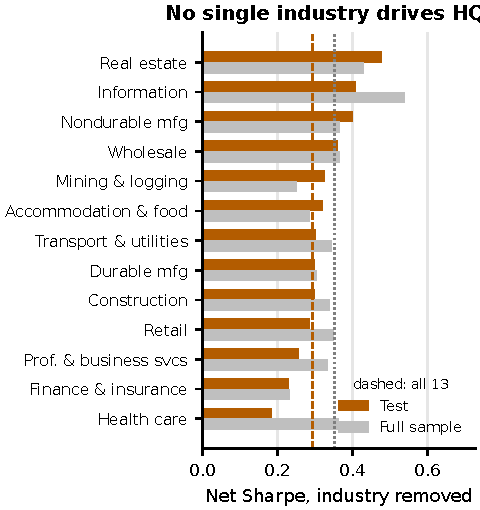
\includegraphics[width=0.55\linewidth]{../report/figures/fig_v2d_dropone.pdf}
\caption{No single industry carries V2d: removing any one leaves the test Sharpe between $+0.18$ and $+0.48$. \textcolor{mute}{\footnotesize Source: v3\_r7\_dropone.csv.} \hfill \tagp}\end{figure}
{\footnotesize\setlength{\tabcolsep}{4pt}% POST-HOC | source: analysis/output/study2/tables/v3_r7_dropone_summary.csv (generated by analysis/run.ipynb)
\begin{tabular}{lrr}
\toprule
statistic & Test Sharpe & Full Sharpe \\
\midrule
minimum & +0.18 & +0.23 \\
median & +0.30 & +0.34 \\
maximum & +0.48 & +0.54 \\
all 13 groups (HQ12) & +0.29 & +0.35 \\
industry whose removal lowers test Sharpe most & Health care &  \\
industry whose removal raises test Sharpe most & Real estate &  \\
\bottomrule
\end{tabular}
}\par\medskip
\subsection*{R8 Tightness moderator \hfill \tagp}
\begin{figure}[H]\centering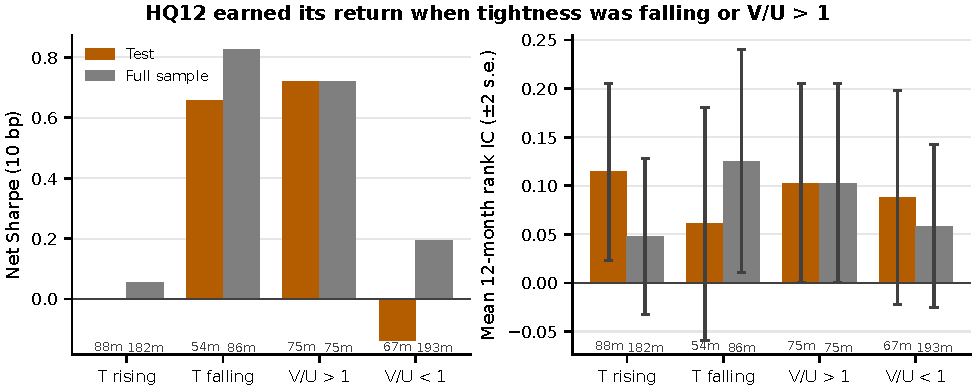
\includegraphics[width=\linewidth]{../report/figures/fig_v2d_tightness.pdf}
\caption{V2d earned its return when tightness was falling or $V/U>1$; in tightening months the Sharpe was zero although the 12-month IC was highest. \textcolor{mute}{\footnotesize Source: v3\_r8\_tightness.csv.} \hfill \tagp}\end{figure}
{\footnotesize\setlength{\tabcolsep}{4pt}% POST-HOC | source: analysis/output/study2/tables/v3_r8_tightness.csv (generated by analysis/run.ipynb)
\begin{tabular}{lrrrr}
\toprule
Months & Sharpe & Net p.a. & IC 12m (t) \\
\midrule
88 & $-$0.00 & $-$0.0\% & +0.115 (+2.52) \\
54 & +0.66 & +6.8\% & +0.061 (+1.02) \\
75 & +0.72 & +6.0\% & +0.103 (+2.00) \\
67 & $-$0.14 & $-$1.2\% & +0.088 (+1.59) \\
182 & +0.06 & +0.4\% & +0.048 (+1.19) \\
86 & +0.83 & +7.6\% & +0.126 (+2.19) \\
75 & +0.72 & +6.0\% & +0.103 (+2.00) \\
193 & +0.19 & +1.4\% & +0.059 (+1.40) \\
\bottomrule
\end{tabular}
}\par\medskip
\subsection*{R9 Block-bootstrap interval \hfill \tagp}
{\footnotesize\setlength{\tabcolsep}{4pt}% POST-HOC | source: analysis/output/tables/v3_r9_bootstrap.csv (generated by analysis/run.ipynb)
\begin{tabular}{lrrrr}
\toprule
Window & Sharpe & 90\% interval & Months & Excludes 0 \\
\midrule
test & +0.29 & [$-$0.07, +0.65] & 142 & no \\
full & +0.35 & [+0.05, +0.64] & 268 & yes \\
\bottomrule
\end{tabular}
}\par\medskip
\subsection*{R10 As-known data \hfill \tagp}
{\footnotesize\setlength{\tabcolsep}{4pt}% POST-HOC | source: analysis/output/tables/v3_r10_asknown.csv (generated by analysis/run.ipynb)
\begin{tabular}{p{4.2cm}p{2.6cm}p{8.6cm}}
\toprule
check & status & note \\
\midrule
R10 as-known (ALFRED vintage) rerun of V2a-V2d & not run: no key & analysis/.env has no FRED\_API\_KEY; historical v2/v3 results use revised data with fixed lags (data\_vintage.md) \\
\bottomrule
\end{tabular}
}\par\medskip
\subsection*{R11 Fundamental law, test window \hfill \tagc\ (A3) / \tagp}
{\footnotesize\setlength{\tabcolsep}{4pt}% CONFIRMATORY (A3) / POST-HOC | source: analysis/output/tables/v3_r11_fundamental_law.csv (generated by analysis/run.ipynb)
\begin{tabular}{lrrrrrrr}
\toprule
Book (test window) & IC & Horizon & BR/yr & TC & Implied IR & Ceiling (TC=1) & Realised Sharpe \\
\midrule
A3 primary & $-$0.021 & 1m & 156 & 0.80 & $-$0.21 & $-$0.27 & $-$0.58 \\
V2a wage growth & +0.049 & 1m & 156 & 0.91 & +0.56 & +0.62 & +0.16 \\
V2d -(hires+quits) 12m & +0.096 & 12m & 13 & 0.48 & +0.17 & +0.35 & +0.29 \\
\bottomrule
\end{tabular}
}\par\medskip
\subsection*{Deflated Sharpe at 112 and 132 trials \hfill \tagp}
{\footnotesize\setlength{\tabcolsep}{4pt}% POST-HOC | source: analysis/output/study2/tables/v3_dsr132.csv (generated by analysis/run.ipynb)
\begin{tabular}{llrrr}
\toprule
Window & DSR (112 trials) & DSR (132 trials) & Benchmark Sharpe (132) \\
\midrule
test & 0.02 & 0.02 & 0.76 \\
full & 0.03 & 0.03 & 0.56 \\
test & 0.00 & 0.00 & 0.76 \\
full & 0.00 & 0.00 & 0.56 \\
test & 0.09 & 0.08 & 0.76 \\
full & 0.16 & 0.15 & 0.56 \\
test & 0.06 & 0.05 & 0.76 \\
full & 0.18 & 0.16 & 0.56 \\
\bottomrule
\end{tabular}
}\par\medskip
\subsection*{Reading rule \hfill \tagp}
{\footnotesize\setlength{\tabcolsep}{4pt}% POST-HOC | source: analysis/output/tables/v3_reading.csv (generated by analysis/run.ipynb)
\begin{tabular}{lr}
\toprule
condition & holds \\
\midrule
R1 hires-only and quits-only test Sharpe > 0 & yes \\
R2 test 12m IC t >= 2 and 1m IC t < 2 & yes \\
R3 holding 9 and 18 months test Sharpe > 0 & yes \\
R4 both test halves Sharpe > 0 & no \\
R5 test break-even cost > 25 bp & yes \\
R7 minimum drop-one test Sharpe > 0 & yes \\
R9 90\% interval excludes 0 (test or full) & yes \\
\bottomrule
\end{tabular}
}\par\medskip
